


\section{What is the Earth System Modeling Framework?}

The Earth System Modeling Framework (ESMF) is a suite of software
tools for developing high-performance, multi-component Earth science
modeling applications.  Such applications may include a few or dozens
of components representing atmospheric, oceanic, terrestrial, or
other physical domains, and their constituent processes (dynamical, chemical,
biological, etc.).  Often these components are developed by different
groups independently, and must be ``coupled'' together using software
that transfers and transforms data among the components in order to form
functional simulations.

ESMF supports the development of these complex applications in a number
of ways.  It introduces a set of simple, consistent component interfaces
that apply to all types of components, including couplers themselves.  These
interfaces expose in an obvious way the inputs and outputs of each component.
It offers a variety of data structures for transferring data between components, 
and libraries for regridding, time advancement, and other common modeling
functions.  Finally, it provides a growing set of tools for using metadata
to describe components and their input and output fields.  This capability
is important because components that are self-describing
can be integrated more easily into automated workflows, model and dataset
distribution and analysis portals, and other emerging ``semantically enabled''
computational environments.

ESMF is not a single Earth system model into which all components
must fit, and its distribution doesn't contain any scientific code.
Rather it provides a way of structuring components so that they can be used 
in many different user-written applications and contexts with minimal code
modification, and so they can be coupled together in new configurations
with relative ease.  The idea is to create many components across a
broad community, and so to encourage new collaborations and combinations.

ESMF offers the flexibility needed by this diverse user base.  It is tested
nightly on more than two dozen platform/compiler combinations; can be
run on one processor or thousands; supports shared and distributed memory
programming models and a hybrid model; can run components
sequentially (on all the same processors) or concurrently (on mutually
exclusive processors); and supports single executable or multiple
executable modes.

ESMF's generality and breadth of function can make it daunting for the
novice user.  To help users navigate the software, we try to apply
consistent names and behavior throughout and to provide many examples.
The large-scale structure of the software is straightforward.
The utilities and data structures for building modeling components 
are called the ESMF {\it infrastructure}.  The coupling interfaces and
drivers are called the {\it superstructure}.  User code sits between
these two layers, making calls to the infrastructure
libraries underneath and being scheduled and synchronized by the 
superstructure above.  The configuration resembles a sandwich, as
shown in Figure~\ref{fig:TheESMFwich}.

ESMF users may choose to extensively rewrite their codes
to take advantage of the ESMF infrastructure, or they may decide to
simply wrap their components in the ESMF superstructure in order to
utilize framework coupling services.  Either way, we encourage users
to contact our 
\htmladdnormallink{support team}{mailto:esmf\_support@ucar.edu}
 if questions arise about how to best
use the software, or how to structure their application.  ESMF is
more than software;  it's a group of people dedicated to realizing
the vision of a collaborative model development community that spans
institutional and national bounds.



\section{The ESMF Reference Manual for Fortran}

ESMF provides a complete set of Fortran interfaces and
some C and C++ interfaces.  This {\it ESMF Reference Manual} is a listing of 
ESMF standard interfaces for Fortran.\footnote{Since the audience for it is 
small, we have not yet prepared a comprehensive reference manual for C 
or C++.}  

Interfaces are grouped by class.  A class is an object-oriented software 
design construct that embodies 
a specific concept like a physical field.  Superstructure classes 
are listed first in this {\it Manual}, followed by infrastructure 
classes.

The major classes in the ESMF superstructure are Components, which 
typically represent
large pieces of functionality such as models, model couplers, and 
dynamics and physics packages; and States, which are the data structures
used to communicate data between Components.  There are both data
structures and utilities in the ESMF 
infrastructure; classes include Fields, collections of Fields on the 
same grid (called Bundles), Arrays, and utilities for communication,
decomposition, time management, and application configuration.

\begin{center}
\begin{figure}
\caption{Schematic of the ESMF ``sandwich'' architecture. In this
design the framework consists of two parts, an upper level
{\bf superstructure} layer and a lower-level {\bf infrastructure} layer.
User code is sandwiched between these two layers.}
\label{fig:TheESMFwich}
\scalebox{1.0}{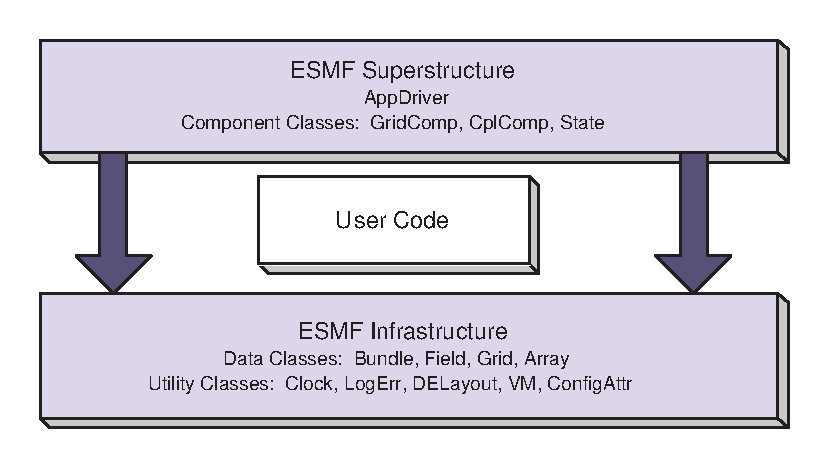
\includegraphics{ESMF_sandwich}}
\end{figure}
\end{center}

